\documentclass[twocolumn, 10pt]{article}
\usepackage[utf8]{inputenc}
\usepackage[T1]{fontenc}
\usepackage{lmodern}
\usepackage{listings}
\usepackage{makeidx}
\usepackage[toc, page]{appendix}
\usepackage{float}
\usepackage{lscape}
\usepackage{csquotes}
\usepackage{soul}
\usepackage{textcomp}
\usepackage{gensymb}
\usepackage{pdfpages}
\usepackage{caption}
\usepackage{subcaption}
\usepackage{url}
\lstset{
	keywords={SELECT, WHERE, COLUMNS, ROWS, ON, MEMBER, WITH, FROM, ALL, CROSSJOIN, TOPCOUNT, ASC, DESC, AS, PARENT, CURRENTMEMBER, CHILDREN, PREVMEMBER, NEXTMEMBER, ORDER, RANK, GENERATE},
	keywordstyle=\color{red}\bfseries
}
% \usepackage{geometry}
\usepackage[left=20mm, right=20mm, top=25mm, bottom=25mm]{geometry}
\usepackage{rotating}
\usepackage[section]{placeins}
\usepackage{chngcntr,array}
\usepackage{graphicx}
\usepackage{lscape}
\usepackage{dirtree}
\usepackage[
	breaklinks=true,
	colorlinks=true,
	linkcolor=blue,
	urlcolor=blue,
	citecolor=blue,
	bookmarks=true,
	bookmarksopenlevel=2
]{hyperref}
\usepackage{xcolor}
\usepackage{algorithm}
\usepackage{algpseudocode}
\usepackage{amsmath}
\usepackage{amsfonts}
\usepackage{amssymb}
\usepackage{indentfirst}

\title{
	Machine Learning
	\\-\\
	Unsupervised Learning and Dimensionality Reduction
}
\author{
	\href{mailto:brandon.alves@gatech.edu}{Brandon Alves}
}
\date{\today}

\begin{document}
	\maketitle
	\thispagestyle{empty}
	\tableofcontents
	% \listoffigures
	% \clearpage
	% \setcounter{page}{1}
	\section{Introduction}
		In this article, I will focus on dimensionality reduction and clustering. I will apply clustering algorithms on two datasets and describe the results. I will also apply dimensionality reduction algorithms on the same datasets and see how the clustering algorithms perform on the reduced datasets. I will also discuss the results of the dimensionality reduction algorithms. Finally I will run one more time my Neural Network learner on the projected data and see how it performs differently.
	\section{Datasets}
		\subsection{Iris Dataset}
			The Iris dataset is a multivariate dataset that contains 150 observations of iris flowers. The dataset contains 4 features: sepal length, sepal width, petal length, and petal width. The dataset also contains the class of each observation, which is the species of the flower. I found this dataset interesting because of the low dimension space it covers, allowing me to easely plot understandable 2D figures to show the results of clustering and dimension reduction algorithms. Also the classes are pretty well separated so we can suppose that clustering algorithms will perform well on this dataset. Figure \ref{fig:iris_org} shows the distribution of the classes in the dataset. We can see that the classes are well separated so we can suppose that clustering algorithms will perform well on this dataset.

			\begin{figure}[h]
				\centering
				\begin{subfigure}[t]{.49\columnwidth}
					\centering
					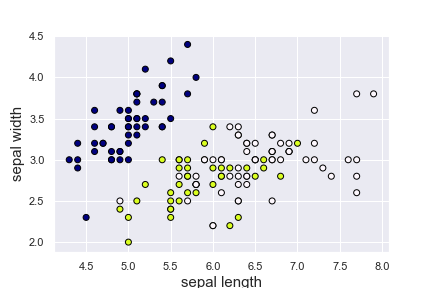
\includegraphics[width=\linewidth]{../graphics/org_sepal_length_sepal_width_label.png}
					\caption{Classes repartition according to sepal length and width}
					\label{fig:iris_org_sep}
				\end{subfigure}
				\begin{subfigure}[t]{.49\columnwidth}
					\centering
					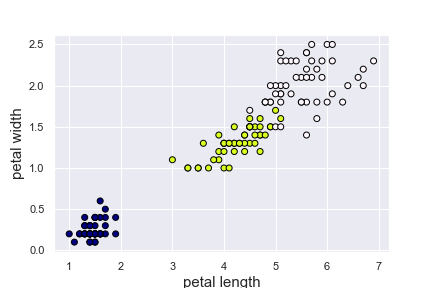
\includegraphics[width=\linewidth]{../graphics/org_petal_length_petal_width_label.png}
					\caption{Classes repartition according to petal length and width}
					\label{fig:iris_org_pet}
				\end{subfigure}
				\caption{Repartition of the classes on Iris dataset according to different parameters}
				\label{fig:iris_org}
			\end{figure}
		\subsection{Gender Dataset}
			The Gender dataset describes some appearence characteritics. It contains 7 features and two classes. The features are: long hair, width of the forehead, height of the forehead, wide nose, long nose, thin lips and the distance between nose and lips. The classes are male and female. I find this dataset interesting because of the high dimension space it covers. So I suspect dimensionality reduction to have an impact on the results  It is also interesting because the classes are not well separated, which means that clustering algorithms will probably not perform well on this dataset. Figure \ref{fig:g_org} shows the distribution of the classes in the dataset according to different features. We can see that some features are more discriminant than others.

			\begin{figure}[h]
				\centering
				\begin{subfigure}[t]{.49\columnwidth}
					\centering
					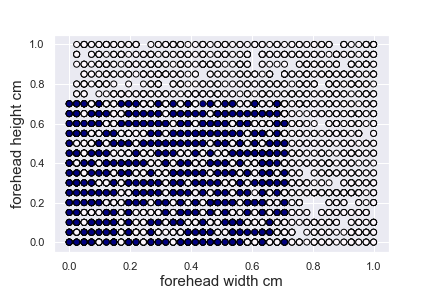
\includegraphics[width=\linewidth]{../graphics/org_forehead_width_cm_forehead_height_cm_label.png}
					\caption{Classes repartition according to forehead width and height}
					\label{fig:g_org_for}
				\end{subfigure}
				\begin{subfigure}[t]{.49\columnwidth}
					\centering
					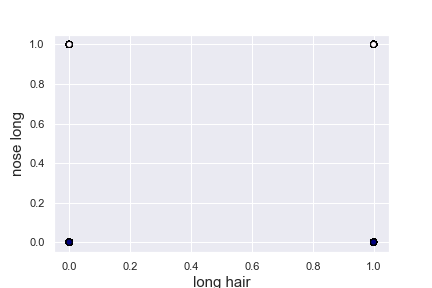
\includegraphics[width=\linewidth]{../graphics/org_long_hair_nose_long_label.png}
					\caption{Classes repartition according to long hair and long nose}
					\label{fig:g_org_hair}
				\end{subfigure}
				\caption{Repartition of the classes on Gender dataset according to different parameters}
				\label{fig:g_org}
			\end{figure}
	\section{Clustering}
		Both \textit{K-means} and \textit{Expectation Maximization (EM)} gave good results applied to both datasets.
		\subsection{Iris Dataset}
			We present on figure \ref{fig:iris_kmeans} the results of K-means applied on Iris dataset. We can see that KMeans obtain an almost perfect classification result. The typical potatoid shape of K-means clusters is easely distinguishable on figure \ref{fig:iris_kmeans_pet}. This particular bias of K-means is also the reason why it makes some mistakes as we can see on figure \ref{fig:iris_kmeans_sep}.

			\begin{figure}[h]
				\centering
				\begin{subfigure}[t]{.49\columnwidth}
					\centering
					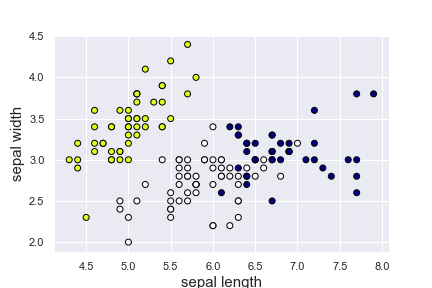
\includegraphics[width=\linewidth]{../graphics/kmeans_sepal_length_sepal_width_label.png}
					\caption{Classes repartition according to sepal length and width}
					\label{fig:iris_kmeans_sep}
				\end{subfigure}
				\begin{subfigure}[t]{.49\columnwidth}
					\centering
					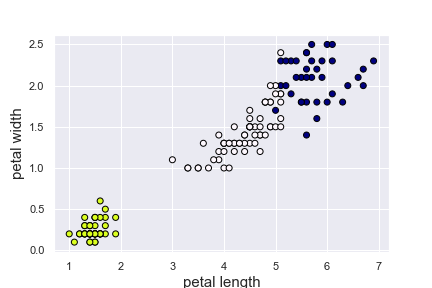
\includegraphics[width=\linewidth]{../graphics/kmeans_petal_length_petal_width_label.png}
					\caption{Classes repartition according to petal length and width}
					\label{fig:iris_kmeans_pet}
				\end{subfigure}
				\caption{Repartition of the K-means clustering results on Iris dataset according to different parameters}
				\label{fig:iris_kmeans}
			\end{figure}

			EM performs even better than kmeans on Iris dataset. We can notice some mistakes on the edges between blue and white areas that are visible on figure \ref{fig:iris_EM_pet}. That is not surprising as the two clusters are very close on every dimensions. In addtion we can note that given it's nature EM let more the blue and white cluster to mix together on figure \ref{fig:iris_EM_sep}. This is due to the large space between points in these parts of the two clusters.

			\begin{figure}[h]
				\centering
				\begin{subfigure}[t]{.49\columnwidth}
					\centering
					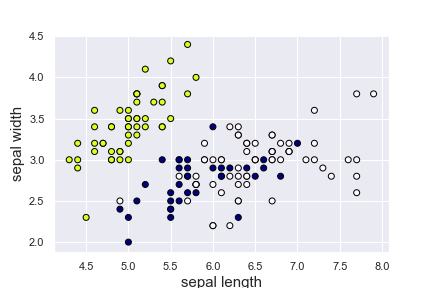
\includegraphics[width=\linewidth]{../graphics/EM_sepal_length_sepal_width_label.png}
					\caption{Classes repartition according to sepal length and width}
					\label{fig:iris_EM_sep}
				\end{subfigure}
				\begin{subfigure}[t]{.49\columnwidth}
					\centering
					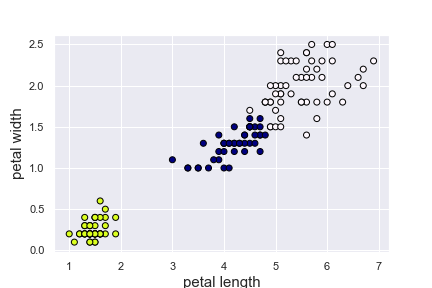
\includegraphics[width=\linewidth]{../graphics/EM_petal_length_petal_width_label.png}
					\caption{Classes repartition according to petal length and width}
					\label{fig:iris_EM_pet}
				\end{subfigure}
				\caption{Repartition of the EM clustering results on Iris dataset according to different parameters}
				\label{fig:iris_EM}
			\end{figure}

			Such good results are not surprising for Iris dataset as it is really a toy dataset for clustering. But I think it gave me a good overview on how the two algorithms work.
		\subsection{Gender Dataset}
			We present on figure \ref{fig:g_kmeans} the results of K-means applied on Gender dataset. K-means perfectly separated most of the data but obtained some errors on the features that are "ambiguous". For example, the hair length and the nose length are a good features to separate the classes as we can see on figure \ref{fig:g_kmeans_pet}. On the other side K-means made some mistakes on the features that are not so discriminant. For example, the forehead width and height are not discriminant at all and we can see on figure \ref{fig:g_kmeans_pet} that K-means made some mistakes on these features. That can be explained by the fact that K-means specifically assumes that the clustering is spherical, which means that each dimension is weighted equally important, and that the clustering problem is an hard clustering problem, meaning that each data point can only belong to one label. However both assumptions are not verified here. Typically the forehead width and height are less important than other dimensions.

			\begin{figure}[h]
				\centering
				\begin{subfigure}[t]{.49\columnwidth}
					\centering
					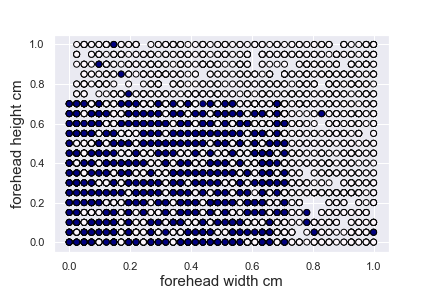
\includegraphics[width=\linewidth]{../graphics/kmeans_forehead_width_cm_forehead_height_cm_label.png}
					\caption{Classes repartition according to forehead width and height}
					\label{fig:g_kmeans_sep}
				\end{subfigure}
				\begin{subfigure}[t]{.49\columnwidth}
					\centering
					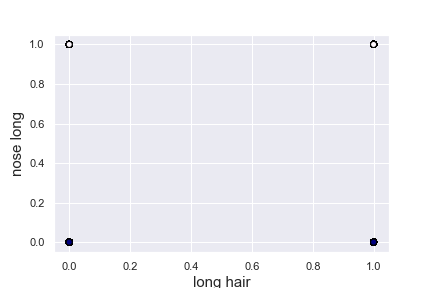
\includegraphics[width=\linewidth]{../graphics/kmeans_long_hair_nose_long_label.png}
					\caption{Classes repartition according to long hair and long nose}
					\label{fig:g_kmeans_pet}
				\end{subfigure}
				\caption{Repartition of the K-means clustering results on Gender dataset according to different parameters}
				\label{fig:g_kmeans}
			\end{figure}

			EM performs better than K-means again on the Gender dataset. Results are pretty similar to K-means. However, as we can see on figure \ref{fig:g_EM_sep}, EM obtain less misclassification than K-means. This can be due to the fact that EM is a soft clustering algorithm, meaning that each data point can belong to multiple labels as they have a probability associated to each label. It allows EM to to get better results here.

			\begin{figure}[h]
				\centering
				\begin{subfigure}[t]{.49\columnwidth}
					\centering
					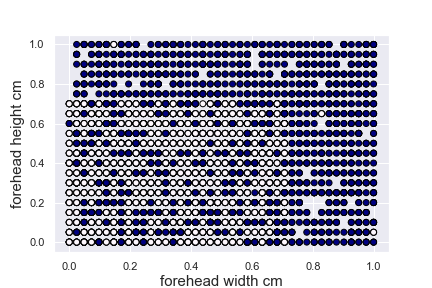
\includegraphics[width=\linewidth]{../graphics/EM_forehead_width_cm_forehead_height_cm_label.png}
					\caption{Classes repartition according to forehead width and height}
					\label{fig:g_EM_sep}
				\end{subfigure}
				\begin{subfigure}[t]{.49\columnwidth}
					\centering
					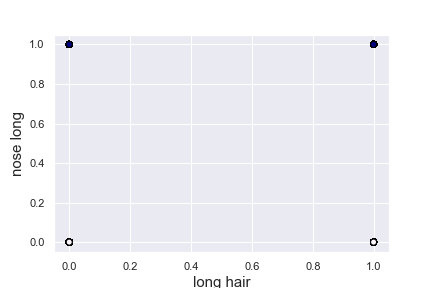
\includegraphics[width=\linewidth]{../graphics/EM_long_hair_nose_long_label.png}
					\caption{Classes repartition according to long hair and long nose}
					\label{fig:g_EM_pet}
				\end{subfigure}
				\caption{Repartition of the EM clustering results on Gender dataset according to different parameters}
				\label{fig:g_EM}
			\end{figure}
		\subsection{Conclusion}
			To conclude, we can say that K-means and EM are two very different algorithms. K-means is a hard clustering algorithm that assumes that the clustering is spherical and that each dimension is weighted equally important. EM is a soft clustering algorithm that does not assume anything on the clustering. However, both algorithms are very efficient and can be used in many different applications. However, we saw that K-means has important biases that can lead to bad results. For example if the each labels would have different densities or if the data is would not have been generated from a spherical distribution.
	\section{Dimensionality Reduction}
		\subsection{Introduction}
			Reducing the number of dimensions of a dataset is a very important task in machine learning especially because of the curse of dimension. In this section, we will present four dimensionality reduction algorithms:
			\begin{itemize}
				\item Principal Component Analysis (PCA)
				\item Linear Discriminant Analysis (LDA)
				\item Randomized Projections (RP)
				\item Linear Discriminant Analysis (LDA)
			\end{itemize}
		\subsection{Principal Component Analysis}
			Something interesting with PCA is that we can rank the selected dimensions according to their eigenvalue. For instance, we can see on figure \ref{fig:pca_score} the eigenvalues and their sum according to the number of dimensions. In both cases, eigenvalues follow an exponentially decrease with the number of dimensions. In the case of Iris dataset, we can notice that one dimension only already give a good description of the dataset as well as in the case of the Gender dataset.

			\begin{figure}[h]
				\centering
				\begin{subfigure}[t]{0.49\columnwidth}
					\centering
					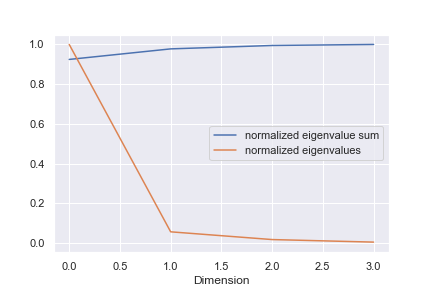
\includegraphics[width=\linewidth]{../graphics/PCA_dimension_importance_4.png}
					\caption{Iris dataset}
					\label{fig:pca_iris_score}
				\end{subfigure}
				\begin{subfigure}[t]{0.49\columnwidth}
					\centering
					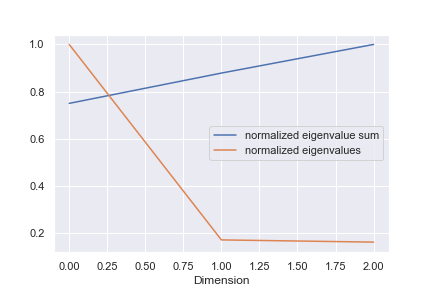
\includegraphics[width=\linewidth]{../graphics/PCA_dimension_importance_3.png}
					\caption{Gender dataset}
					\label{fig:pca_g_score}
				\end{subfigure}
				\caption{Evolution of the score according to the number of dimension for both dataset}
				\label{fig:pca_score}
			\end{figure}

			We can see on figure \ref{fig:pca} the results of the PCA dimensionality reduction on both datasets. In the case of Iris dataset, the 3 classes really appear to be on different areas. We can also see that the first dimension (numbered $0$) is the most important one as it is the one that separates the most the classes. Indeed, the different areas almost seem to be separated by vertical lines. This is coherent with how PCA works and the fact that PCA ranks by importance the chosen dimensions. We have the same results for the Gender dataset. The first dimension is almost discriminant enough to separate the two classes. However, we can notice more mixing between the two classes than in the case of the Iris dataset. But the second dimension does not seem to be usefull enough.

			\begin{figure}[h]
				\centering
				\begin{subfigure}[t]{0.49\columnwidth}
					\centering
					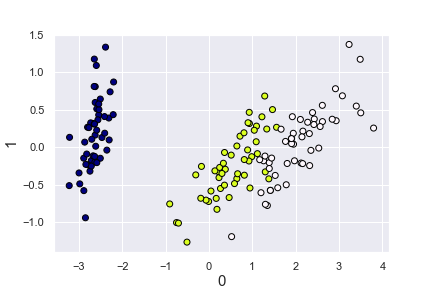
\includegraphics[width=\linewidth]{../graphics/pca_iris_0_1_label.png}
					\caption{Iris dataset}
					\label{fig:pca_iris}
				\end{subfigure}
				\begin{subfigure}[t]{0.49\columnwidth}
					\centering
					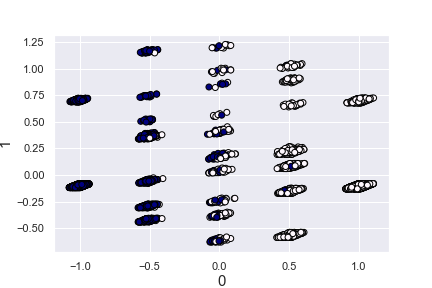
\includegraphics[width=\linewidth]{../graphics/pca_g_0_1_label.png}
					\caption{Starcraft dataset}
					\label{fig:pca_g}
				\end{subfigure}
				\caption{Representation of the classes after projection in the best plan found by PCA}
				\label{fig:pca}
			\end{figure}

			In a clustering point of view, K-means obtained worse results than on the original dataset. This can probably be explained by the fact that K-means considers all dimensions as equally important. However, in this case, we saw that the first dimension is much more discriminant than the second one. EM obtained here almost a perfect result. We obtained similar results for the Gender dataset.

			In conclusion, PCA is a fast and efficient algorithm to reduce the number of dimensions. It also provides a information to rank the dimensions according to their importance.
		\subsection{Independent Component Analysis}
			ICA is a dimensionality reduction algorithm that is based on the assumption that the data is a linear combination of independent sources. The goal of ICA is to find the independent sources that are the most important to describe the data. In this section, we will present the results of ICA on both datasets. In the case of the Iris dataset, we can see on figure \ref{fig:ica_iris} that the results are verry similar to those from PCA. If we perform an axial symmetry by an horizontal line on the top of the figure, we get the nearly the same results as for PCA. Thus, we can apply the same conclusion than for PCA here. However, it is important to notice that the scale is different. For ICA, the ratio of the range of axis 0 over the range of axis 1 is about 0.7, while it was 2.4 for PCA, explaining the clustering difference. For the Gender dataset, we obtained exactly the same transformation as for PCA as we can see on figure \ref{fig:ica_g}.

			\begin{figure}[h]
				\centering
				\begin{subfigure}[t]{0.49\columnwidth}
					\centering
					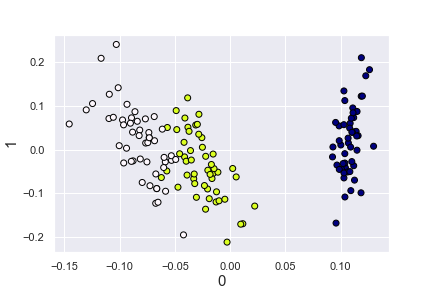
\includegraphics[width=\linewidth]{../graphics/ica_iris_0_1_label.png}
					\caption{Iris dataset}
					\label{fig:ica_iris}
				\end{subfigure}
				\begin{subfigure}[t]{0.49\columnwidth}
					\centering
					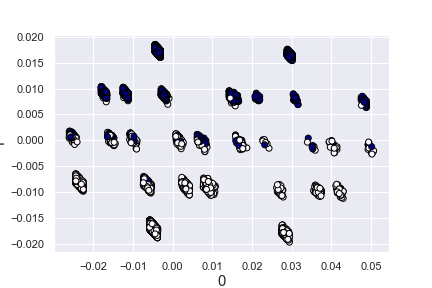
\includegraphics[width=\linewidth]{../graphics/ica_g_0_1_label.png}
					\caption{Gender dataset}
					\label{fig:ica_g}
				\end{subfigure}
				\caption{Representation of the classes after projection in the best plan found by ICA}
				\label{fig:ica}
			\end{figure}

			In a clustering perspective, due to the change of proportions, both K-means and EM wrongly split the two clusters on the right for the Iris dataset and split them horizontally intead of vertically. In addition, K-means managed to misclassify one point in the left cluster. Like for PCA, the dimension 0 is the one with the more information. Reducing its amplitude regarding to the other dimension results in giving more importance to that last dimension. For the Gender dataset, the results are again coherent with the ones from Iris. Both K-means and EM obtained poor results. EM is the most impacted by this change of scale. Which seems fair as we know that EM does not assume any equal importance between dimensions.

			In conclusion, ICA gave very similar results than PCA. However, because of the difference of scale it gave very poor results on clustering.
		\subsection{Randomized Projections}
			Randomized Projections (RP) is a time efficient algorithm to reduce dimensions. Its random specificity let us exoect worse results than the methods above. On the Iris dataset, RP gave average results. We can see on Figure \ref{fig:rnd_iris} that the global shape is close to the shape obtained by PCA and ICA, with one cluster far from the two others which are very close. This projection is far from optimal in a clustering point of view, but the clusters are still there. For the Gender dataset, results are more chaotic. We can see on Figure \ref{fig:rnd_g} that the two classes are mixed together. Moreover, the algorithm is not stable as the results are different each time we run it. This is due to the random nature of the algorithm.

			\begin{figure}[h]
				\centering
				\begin{subfigure}[t]{0.49\columnwidth}
					\centering
					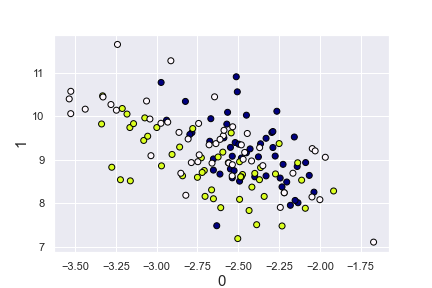
\includegraphics[width=\linewidth]{../graphics/rnd_iris_0_1_label.png}
					\caption{Iris dataset}
					\label{fig:rnd_iris}
				\end{subfigure}
				\begin{subfigure}[t]{0.49\columnwidth}
					\centering
					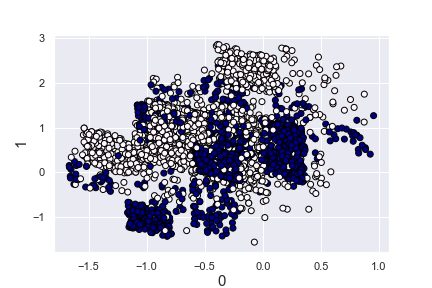
\includegraphics[width=\linewidth]{../graphics/rnd_g_0_1_label.png}
					\caption{Gender dataset}
					\label{fig:rnd_g}
				\end{subfigure}
				\caption{Representation of the classes after projection in a plan by random projection}
				\label{fig:rnd}
			\end{figure}

			In a clustering point of view, K-means and EM obtained very poor results in the case of Iris dataset as well as in the case of the Gender dataset. Either K-means and EM are impacted by the poor dimension reduction operated by RP algorithm.

			Therefore, RP does not obtained good results on applying clustering algorithms. Except its low time complexity, like using it as a reference to evaluate the performance of other dimension reduction algorithms, we did not see its interest on both datasets.
		\subsection{Linear Discriminant Analysis}
			LDA is different from the other dimensions reduction algorithms we have seen so far. It is the only one to include the labels in order to chose the best projection. This fact transforms the clustering into a supervised problem. That makes LDA biased toward the labels we are looking for. This bias is interesting here to see how this information change the results, but usually clustering is used when we do not know what we are looking for, case where LDA is inappropriate.

			We can see on figure \ref{fig:lda_iris} the projection of the Iris dataset onto two dimensions. We can see that the two classes are well separated. Two classes are still near from each other, but that is coherent with the original data. We can also look at the range ratio, but it will not be useful as axis 0 already give most of the information needed to correctly classify the data, as long as this ration stay near 1, we can expect good clustering results later. Therefore, LDA projects the Iris dataset into nearly one dimension, showing that with only a linear combination of the variable we have enough information to find all the classes of this dataset. LDA does not permit to project in more than one dimension in the case of the Gender dataset, as we can see on figure \ref{fig:lda_g}. The projection is pretty good as the two classes are well separated.

			\begin{figure}[h]
				\centering
				\begin{subfigure}[t]{0.49\columnwidth}
					\centering
					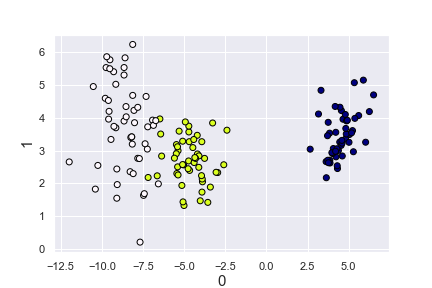
\includegraphics[width=\linewidth]{../graphics/lda_iris_0_1_label.png}
					\caption{Iris dataset}
					\label{fig:lda_iris}
				\end{subfigure}
				\begin{subfigure}[t]{0.49\columnwidth}
					\centering
					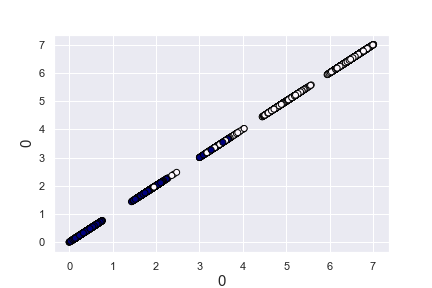
\includegraphics[width=\linewidth]{../graphics/lda_g_0_0_label.png}
					\caption{Gender dataset}
					\label{fig:lda_g}
				\end{subfigure}
				\caption{Representation of the classes after projection in the best plan found by LDA}
			\label{fig:lda}
			\end{figure}

			The clustering on the Iris dataset after projection is pretty good. Both K-means and EM obtained almost perfect results. There is some erros on the borders of two close clusters, but in a smaller way than what we have seen before. They get much less confused by the second dimension, probably because it ranges on a smaller interval than the first one. For the Gender dataset, the clustering is also good. Again there is some errors but it is interesting to see that only one dimension was actually needed to separate the two classes.

			Finally, LDA did a good job in both datasets. In addition for this little improvement in comparison with other algorithms such as PCA and ICA, LDA comes with the cost of needing the labels. It is so not used in the same cases than the other algorithms. However, it is interesting to see how the labels can help to find the best projection. While the other algorithms are useful when we do not know what we are looking for, LDA is useful when we know what we are looking for and just want to reduce the dimensionality before running classification algorithm for example.
		\subsection{Conclusion}
			We have seen that applying dimension reduction before clustering can be very efficient to compress data dimensions while keeping them as meaningful as possible. This can also be very useful to limit the effect of the curse of dimensionality.

			I did not discussed runtime in that section. In fact most of them are very low. All algorithms complete their execution in less than few seconds. It is also the case for K-means. EM is however much slower. Thus, if EM generally performed better than K-means, it must be underlined that it is much slower. That fact could explain why K-means is still very popular.

			I apologies for the lack of figures in this section, due to space constraint I had to make some sacrifices. Thus the plots of the different clusters were not included but are available in the code repository.
	\section{Training a Neural Network after Dimensionality Reduction}
		\subsection{Introduction}
			Feature selection applied before using a classifier is a common practice to limit the effect of the curse of dimensionality. We can expect that reducing the number of dimensions will reduce the accuracy of our neural network and reduce its convergence time.

			Like in the previous homeworks, the hard line of the plots represents the median value while the hue area goes from the minimum to the maximum value. The neural network structure is described as follows: $(a)$ represents a perceptron with one hidden layer of $a$ neurons and $(a, b)$ represents a perceptron with two hidden layers of $a$ and $b$ neurons respectively.

			I will use here the same dataset as in the homework 1 as well as the same network structure. I set most of the parameters explored the same as in homework 1.  For instance, I used batch normalization in all the experiment, as well as the rmsprop optimizer from Keras. Thus, the reader can easily compare the actual results with the previous ones. I will also explore some new parameters such as the dimensionality reduction algorithm, the number of dimensions kept and the shape of the hidden layers. The dimensionality reduction was first fit on the train dataset and then applied to both train and test data. Repartition between train and test reminded the same as in the first assignment.

			We can see on figure \ref{fig:per_all_rm} that not all the different dimensionality reduction algorithms converge to the same accuracy. RP gave the the worst results while PCA, ICA and LDA gave the same median accuracy. We can also notice that RP is the slowest method that converges according to the number of epochs while LDA is the fastest. It is also interesting to notice that on figure \ref{fig:per_all_nf}, the dataset with a number of dimension reduced to one is the fastest to converge while the one reduced to 6 dimension is the third fastest. Here they all converge to the same accuracy, which is the purpose of feature selection: reducing the number of dimensions without losing too much information. However the median accuracy is a little bit lower than without feature selection if we recall homework 1. Although the median accuracy is the same, we have to note that the minimum accuracy happens to reach 0.5 in the case of 1 feature with RP and 3 features with ICA.

			Let's now study the specific results for each dimensionality reduction algorithm.
			\begin{figure}[h]
				\centering
				\begin{subfigure}[t]{0.7\columnwidth}
					\centering
					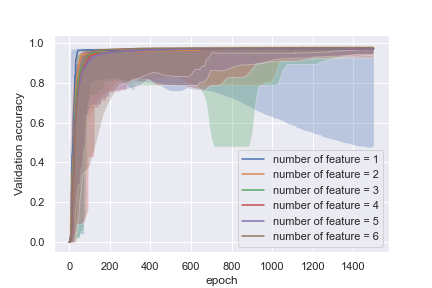
\includegraphics[width=\linewidth]{../graphics/all_epoch_val_categorical_accuracy_number_of_feature.png}
					\caption{Effect of the number of feature}
					\label{fig:per_all_nf}
				\end{subfigure}
				\begin{subfigure}[t]{0.7\columnwidth}
					\centering
					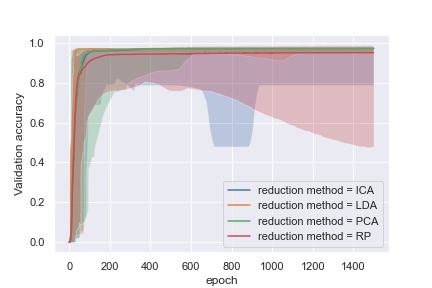
\includegraphics[width=\linewidth]{../graphics/all_epoch_val_categorical_accuracy_reduction_method.png}
					\caption{Effect of the reduction method used}
					\label{fig:per_all_rm}
				\end{subfigure}
				\caption{Validation accuracy according to the epoch for all the different combination}
				\label{fig:per_all}
			\end{figure}
		\subsection{Principal Component Analysis}
			PCA gave the best results after LDA. We can see on figure \ref{fig:per_pca_nf} that there is much less variation in the accuracy. We can see that all the transformed datasets gave the same accuracy which is a little bit lower than the one without transformation. As expected, PCA with one dimension is the fastest to converge.

			It is interesting to notice that like in homework 1, the layer structure that get fastest convergence is the most complex one : $(30, 10)$. The accuracy is not really affected by the network structure. We can see on figure \ref{fig:per_pca_nf_3525} the effect of the number of features for $(10)$ and $()$ layers. Here we see that the convergence speed highly depends on the number of features. The fastest convergence is given with only one feature and decreases while the features increase.

			We have also notice that the validation accuracy of small layers is rising slower than complex layers. This is probably due to the fact that the bigger weights, the bigger layers are easier to fit into a local optimum. So if we want to approximate a complex function it's easier with lot of simple ones than than with a few of complex ones, even if the later is probably more reliable.

			\begin{figure}[h]
				\centering
				\begin{subfigure}[t]{0.7\columnwidth}
					\centering
					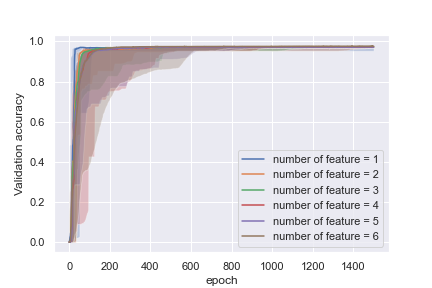
\includegraphics[width=\linewidth]{../graphics/PCA_epoch_val_categorical_accuracy_number_of_feature.png}
					\caption{Effect of the number of features for all tested layers}
					\label{fig:per_pca_nf}
				\end{subfigure}
				\begin{subfigure}[t]{0.7\columnwidth}
					\centering
					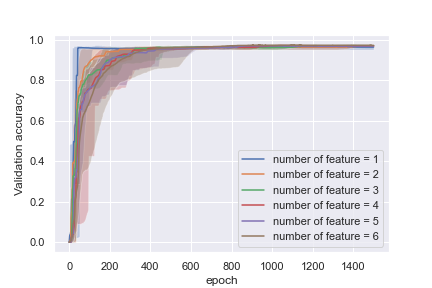
\includegraphics[width=\linewidth]{../graphics/PCA_epoch_val_categorical_accuracy_number_of_feature_10_.png}
					\caption{Effect of the number of features for $(10)$ and $()$ layers}
					\label{fig:per_pca_nf_3525}
				\end{subfigure}
				\caption{Validation accuracy according to the epoch with PCA}
				\label{fig:per_pca}
			\end{figure}

			To conclude, PCA is a good dimensionality reduction algorithm to use with a neural network. The results are not as good as in the original dataset and the converge is a little bit slower. However, the results are still very good and the converge is still very fast. It is important to note that the number of features must be chosen carefully. If too many features are selected, the neural network will tend to overfit on some datasets. On the other hand, if too few features are selected, the neural network will not be able to learn enough to perform well.
		\subsection{Independent Component Analysis}
			The first thing we can notice on figure \ref{fig:per_ica_nf} is that PCA gives the highest variation in terms of accuracy. The median accuracy value is not really affected by the number of features, however, the minimum accuracy is. We can see that it happens, with 3 features, to get a score of only 0.5. ICA assumes that at most one subcomponent is Gaussian and that the subcomponents are statistically independent from each other. The results we get let us think that this assumption is not always true. We can also see that the convergence speed is not really affected by the number of features.

			In figure \ref{fig:per_ica_nf_3525}, we can see that ICA is the only dimensionality reduction algorithm that leads to overfitting. Those results are obtain with the two simplest network structure. Even if there is no overfitting with layers $(30, 10)$, that let us think that ICA is not really well suited for this kind of problem.

			\begin{figure}[h]
				\centering
				\begin{subfigure}[t]{0.7\columnwidth}
					\centering
					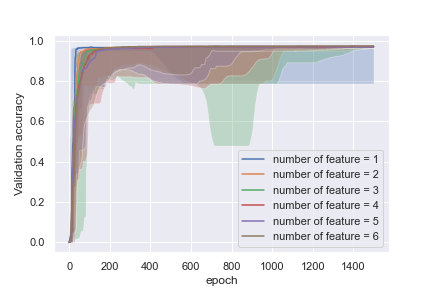
\includegraphics[width=\linewidth]{../graphics/ICA_epoch_val_categorical_accuracy_number_of_feature.png}
					\caption{Effect of the number of features for all tested layers}
					\label{fig:per_ica_nf}
				\end{subfigure}
				\begin{subfigure}[t]{0.7\columnwidth}
					\centering
					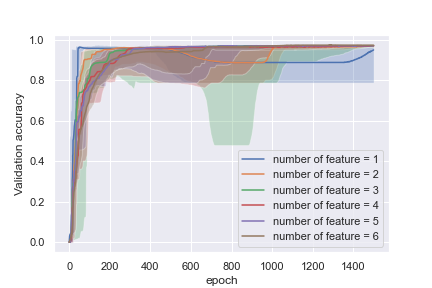
\includegraphics[width=\linewidth]{../graphics/ICA_epoch_val_categorical_accuracy_number_of_feature_10_.png}
					\caption{Effect of the number of features for $(10)$ and $()$ layers}
					\label{fig:per_ica_nf_3525}
				\end{subfigure}
				\caption{Validation accuracy according to the epoch with ICA}
				\label{fig:per_ica}
			\end{figure}

			To conlude, we can say that ICA gave good results but not as good as PCA. If we had to choose between the two, we would choose PCA. So, we consider that ICA is not really relevant in our case, probably because there is no really hidden variable here to discover.
		\subsection{Randomized Projections}
			RP gave the worst results compared to the other methods. We can see on figure \ref{fig:per_rnd_nf} that unlike with the other methods, the accuracy depends on the number of features. The less features we use, the less the accuracy is. However, we get better results with 3 features than with 5. This is the result of being random, but the general
			trend observed is still true, the more features the better the accuracy is.

			Here again the layers which gave the best results are the most complex ones. It definitely seems that feature reduction does not seem to impact the optimal structure of the network.

			On figure \ref{fig:per_rnd_nf_3525}, we can see that that the neural network overfits with the network composed of no hidden layer. This is probably due to the fact that the neural network is not complex enough to learn the function. Hwever in all the other configurations, the neural network does not overfit. It shows that overfitting is not only dependent on the shape of the data and of the network but is also highly dependent on the content of the data. We see that RP did not produce features that were particularly relevant on the train dataset but were completely uncorrelated to the classes in the test dataset. As the results show, that comes with the cost of a lower accuracy.

			\begin{figure}[h]
				\centering
				\begin{subfigure}[t]{0.7\columnwidth}
					\centering
					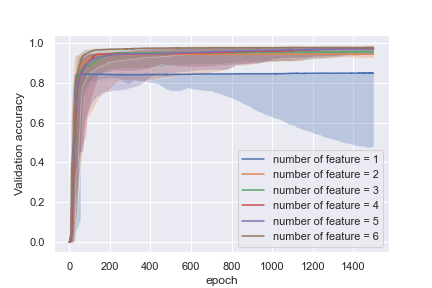
\includegraphics[width=\linewidth]{../graphics/RP_epoch_val_categorical_accuracy_number_of_feature.png}
					\caption{Effect of the number of features for all tested layers}
					\label{fig:per_rnd_nf}
				\end{subfigure}
				\begin{subfigure}[t]{0.7\columnwidth}
					\centering
					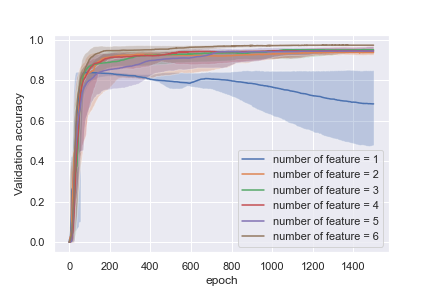
\includegraphics[width=\linewidth]{../graphics/RP_epoch_val_categorical_accuracy_number_of_feature_10_.png}
					\caption{Effect of the number of features for $(10)$ and $()$ layers}
					\label{fig:per_rnd_nf_3525}
				\end{subfigure}
				\caption{Validation accuracy according to the epoch with RP}
				\label{fig:per_rnd}
			\end{figure}

			To conlude, RP is not good as PCA or ICA. But it is very fast. However it can become particularly powerful when it is needed to cut a lot of dimensions efficiently.
		\subsection{Linear Discriminant Analysis}
			LDA is completely in an other hand than the previous dimensionality reduction algorithms. First, because of its supervised approach, in which we say what information we want to keep. As discussed before, this strategy is often problematic, but here I wanted to show the benefits from using it. Second, because of its results. We can see on Figure \ref{fig:per_all_rm} that LDA is the best performer both in accuracy and in convergence speed.

			LDA only results in a number of features equal to the number of classes minus one. So here, we were only able to get one resulting feature. However it is interesting so see that LDA managed to get an accuracy as good as PCA with 6 features. It is this information on labels that give LDA such a pertinence here. In addition, in terms of epoch, the training time of the perceptron is even better than the one obtained with PCA. We can suppose that it will be difficult to be faster than that while reducing the number of dimensions.

			As you can see on figure \ref{fig:per_lda_nf_3525}, best results are also obtained with layers $(30, 10)$ and $(30, 10, 5)$. This is the same as with PCA and ICA. We can deduce that the optimal structure of the network is not impacted by the dimensionality reduction method.

			We can see that the neural network does not overfit with LDA. We could expect overfitting because of the small number of features and the particularity that LDA is a supervised method, but it was not the case. As every supervised algorithm, LDA can overfit and loss its generalization capabilities. Here we trained both LDA and the perceptron on a dataset and computed accuracy on another one, and so we are pleased to see that the transformation learn by LDA is still pertinent on the test dataset.

			\begin{figure}[h]
				\centering
				\begin{subfigure}[t]{0.7\columnwidth}
					\centering
					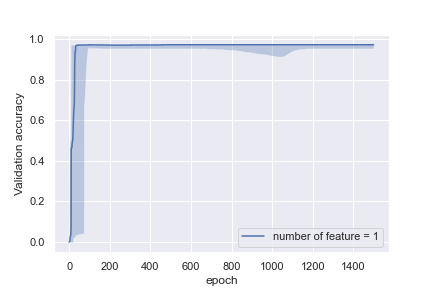
\includegraphics[width=\linewidth]{../graphics/LDA_epoch_val_categorical_accuracy_number_of_feature.png}
					\caption{Effect of the number of features for all tested layers}
					\label{fig:per_lda_nf}
				\end{subfigure}
				\begin{subfigure}[t]{0.7\columnwidth}
					\centering
					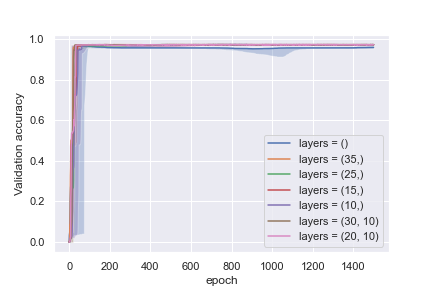
\includegraphics[width=\linewidth]{../graphics/LDA_epoch_val_categorical_accuracy_layers.png}
					\caption{Effect of the layers}
					\label{fig:per_lda_nf_3525}
				\end{subfigure}
				\caption{Validation accuracy according to the epoch with LDA}
				\label{fig:per_lda}
			\end{figure}

			To conclude, LDA allows to quickly reduce the number of dimensions to be used by a learning method, which can help to improve its efficiency. However, it is not always the best method to use, as it is not always possible to know what label we want to learn.
		\subsection{Conclusion}
			In this section, we saw that the learning capability of a neural network can depend on the dimensionality reduction method used. The resulting number of feartures also has an impact on the learning capability of the neural network. We also saw that the optimal structure of the neural network is not impacted by the dimensionality reduction method used. Finally, the number of layers of the neural network does not seem to have an big impact in its accuracy, but principally in its convergence speed. We have shown in the homework one that some parameters can completely reduce the accuracy, the size of the layers does not have as much importance as the information available in the data.
	\section{Adding Clusters as Features}
		\subsection{Introduction}
			In that section, we will try to add clusters as features to the neural network. We will use the K-means algorithm to create clusters and then add them as features to the neural network. We will see if it improves the accuracy of the neural network. Adding that information can provide additional information to the neural network, particularly if some cluster is highly correlated to a given class.

			As a global trend, we can see on figure \ref{fig:clusper_all}, that the best results are a little bit better than the ones in the previous section, with an improvement of 0.02 in accuracy. Another difference, as we can see on figure \ref{fig:clusper_all_rm}, is that every dimensionality reduction method gave very close median results, especially in the convergence speed, which was not the case in the previously.

			We can also see on figure \ref{fig:clusper_all_cm} that while EM was performing better than k-means in section 4, here k-means gets better results no matter the metric we use. That is a good improvement as k-means is much faster than EM.

			\begin{figure}[h]
			\centering
				\begin{subfigure}[t]{0.7\columnwidth}
					\centering
					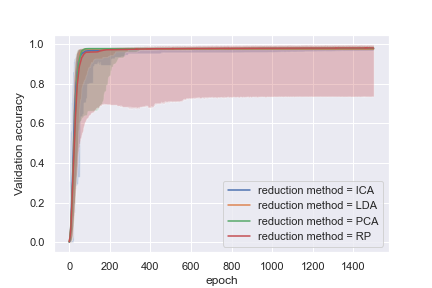
\includegraphics[width=\linewidth]{../graphics/clusper_all_epoch_val_categorical_accuracy_reduction_method.png}
					\caption{Effect of the reduction method on validation accuracy}
					\label{fig:clusper_all_rm}
				\end{subfigure}
				\begin{subfigure}[t]{0.7\columnwidth}
					\centering
					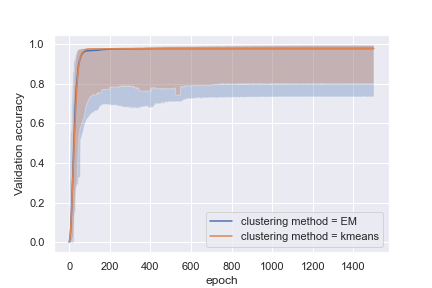
\includegraphics[width=\linewidth]{../graphics/clusper_all_epoch_val_categorical_accuracy_clustering_method.png}
					\caption{Effect of the clustering method on validation accuracy}
					\label{fig:clusper_all_cm}
				\end{subfigure}
				\caption{Validation accuracy according to the epoch when cluster are added as new features}
				\label{fig:clusper_all}
			\end{figure}

			As we can see on figure \ref{fig:clusper_all_layers}, layers are by far the most important parameters here. They all obtain the same accuracy here which was not the case previously. The layer connecting directly input to output neurones gets the worst results as before. This is not surprising as all the other layers try to reduce the number of dimensions in the hidden layers.

			\begin{figure}[h]
				\centering
				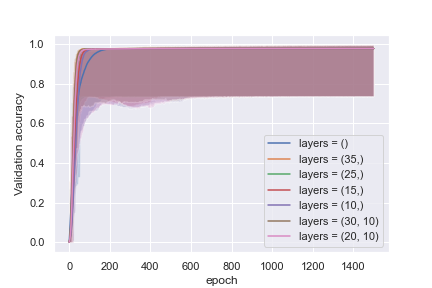
\includegraphics[width=0.7\linewidth]{../graphics/clusper_all_epoch_val_categorical_accuracy_layers.png}
				\caption{Effect of the clustering method on validation accuracy for different layers}
				\label{fig:clusper_all_layers}
			\end{figure}
		\subsection{Principal Component Analysis}
			PCA follows here the general trend, in such a way that we can qualify it as the median dimension reduction algorithm here. Thus it follows all general observation discussed above and give only little advantage to K-means over EM. It also allows k-means to have less variation especially when the number of epochs is low as we can see on figure \ref{fig:clusper_pca_cm}.

			\begin{figure}[h]
				\centering
				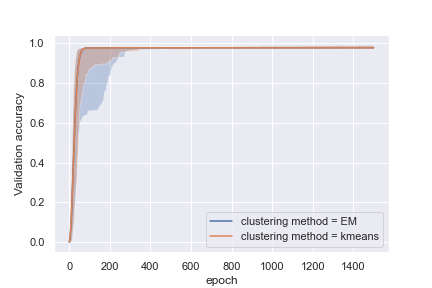
\includegraphics[width=0.7\linewidth]{../graphics/clusper_PCA_epoch_val_categorical_accuracy_clustering_method.png}
				\caption{Effect of the clustering method on validation accuracy when using PCA}
				\label{fig:clusper_pca_cm}
			\end{figure}
		\subsection{Independent Component Analysis}
			As we can see on figure \ref{fig:clusper_ica_cm}, ICA gave results very close to PCA with k-means a little above EM. That time we can notice that we do not have overfitting anymore with ICA. Adding clusters as features seems to help the neural network to avoid overfitting.

			\begin{figure}[h]
				\centering
				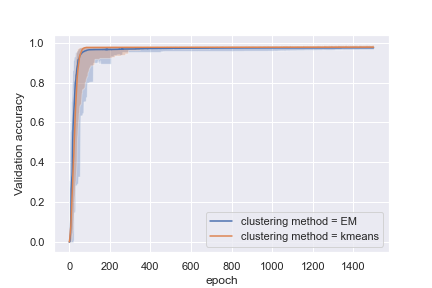
\includegraphics[width=0.7\linewidth]{../graphics/clusper_ICA_epoch_val_categorical_accuracy_clustering_method.png}
				\caption{Effect of the clustering method on validation accuracy when using ICA}
				\label{fig:clusper_ica_cm}
			\end{figure}
		\subsection{Randomized Projections}
			RP is the only method that let the neural network get better results with EM over k-means as we can see on figure \ref{fig:clusper_rnd_cm}. Adding clusters as features also permits RP to get accuracy as good as the other methods. However the variation is still very high. compared to the other methods. It is interesting to get as good results as we saw in previous section that RP method did not give good results with clustering.

			\begin{figure}[h]
				\centering
				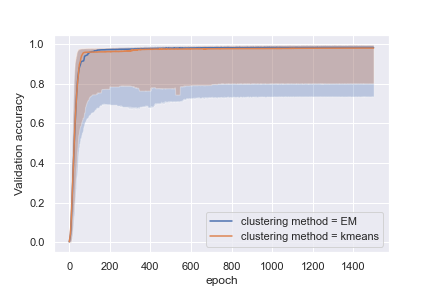
\includegraphics[width=0.7\linewidth]{../graphics/clusper_RP_epoch_val_categorical_accuracy_clustering_method.png}
				\caption{Effect of the clustering method on validation accuracy when using RP}
				\label{fig:clusper_rnd_cm}
			\end{figure}
		\subsection{Linear Discriminant Analysis}
			As we can see on figure \ref{fig:clusper_lda_cm}, with LDA, the difference between k-means and EM is almost zero. The fact that EM does not perform as well as before could be explained by the fact that LDA try to split the data in a K-Means pertinent way that do not take into account the probabilistic vision of EM.

			\begin{figure}[h]
				\centering
				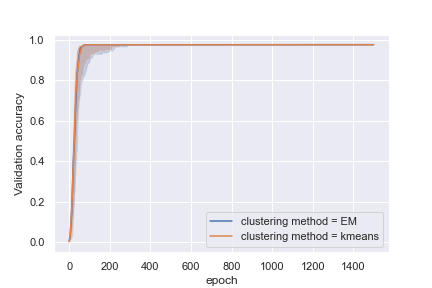
\includegraphics[width=0.7\linewidth]{../graphics/clusper_LDA_epoch_val_categorical_accuracy_clustering_method.png}
				\caption{Effect of the clustering method on validation accuracy when using LDA}
				\label{fig:clusper_lda_cm}
			\end{figure}
		\subsection{Conclusion}
			To conclude, we can say that adding the result of a clustering algorithm as feature for a neural network helps to get better results, at least in our specific case. One explanation of the results we obtained here is that the clusters generated on the train dataset gave good insights to find the desired class and that those clusters extend to the test data set. This conclusion is strengthened by the fact that accuracy on the train data set converge far quicker toward perfect results on this section than on last section. So we can assume that the neural network takes advantage here to learn more efficiently thanks to the cluster information which is coherent from a dataset to the other.
	\section{Conclusion}
		In that report we discovered the benefits and drawbacks of dimensionality reduction methods and clustering algorithms. We saw that dimensionality reduction can be a powerful tool. However not all algorithms are well adapted to all datasets. One difficulty is to find the appropriate method as well as the appropriate number of dimensions to keep. We also saw that clustering algorithms can help find information in the data which is the purpose of data mining. We also explored the possibility to use dimensionality reduction to train a neural network. We saw that even if in a theoretical point of view it is better to have fewer dimensions as input, loss of information happens resulting in a lower accuracy. Finally, we saw that adding the result of a clustering algorithm as feature for a neural network can help to get better results.

		Dimensionality reduction was a concept I have heard of before, but which I never really used before that work. It was very interesting to learn more about, and have a little experience with the different methods we used. It is not the same for clustering as I took a data mining class before. As I had some little experience on it, the different experiments on this concept may seem a little bit light. If that is the case, I apologize for that. I hope that the report is clear enough and that the reader will enjoy reading it.
\end{document}